\documentclass[preview,border=4mm,convert={convertexe={magick},outext=.ps}]{standalone}
\usepackage[dvipdfm]{geometry}

%graphics
\usepackage{xcolor}
\usepackage{tikz}
\usetikzlibrary{shapes.geometric, shapes.multipart, arrows, arrows.meta,calc, through,intersections, circuits.logic.US}
\usepackage[caption=false,font=footnotesize]{subfig}


\begin{document}
\begin{figure}[!t]
\centering

\subfloat[c17 circuit network]{
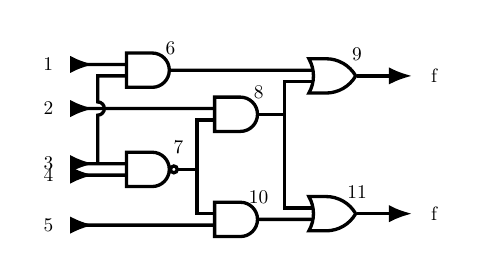
\begin{tikzpicture}[transform shape, scale=0.7, circuit logic US, every node/.style={very thick, minimum size=0.75cm}, very thick]

\node(o1)[or gate, point right]  at (6,3){};
\node(o2)[or gate, point right]  at (6,0.5){};

\node (a1)[and gate, point right] at ($(o1.input 1) - (3,0)$) {};
\node at (a1.output)[above]{6};
\node (a2)[and gate, point right] at ($(o1.input 1) - (1.4,.8)$) {};
\node at (a2.output)[above]{8};
\node (a3)[and gate, point right] at ($(o2.input 2) - (1.4,0)$) {};
\node at (a3.output)[above]{10};
\node (nand1)[nand gate, point right] at ($(a1) - (0,1.8)$){};
\node at (nand1.output)[above]{7};

\draw (o1.input 1) -- (a1.output);
\draw (o1.input 2) -- ++(-0.5,0) |- (a2.output);
\draw (o2.input 2) -- (a3.output);
\draw (o2.input 1) -- ++(-0.5,0) |- (a2.output); 
\draw (a2.input 2) -- ++(-0.3,0) |- (nand1.output);
\draw (a3.input 1) -- ++(-0.3,0) |- (nand1.output);

\draw[>=Latex, ->] (o1.output) node[above]{9} -- +(1,0) node[right]{f};
\draw[>=Latex, ->] (o2.output) node[above]{11} -- +(1,0) node[right]{f};

\coordinate (i1) at ($(a1.input 1) - (1,0)$);
\coordinate (i2) at ($(a2.input 1) - (2.6,0)$);
\coordinate (i3) at ($(nand1.input 1) - (1,0)$);
\coordinate (i4) at ($(nand1.input 2) - (1,0)$);
\coordinate (i5) at ($(a3.input 2) - (2.6,0)$);

% \coordinate (pivot) at ($(a3.input) - (2.6,0)$);
\begin{scope}[>=Latex]
% \draw[>-] (a1.input -| pivot) node(s)[left]{s} -- node[above]{1}(n1.input);
% \draw[>-] (a2.input 1 -| pivot) node(b)[left]{b} --(a2.input 1);
% \draw[>-] (a1.input 1 -| pivot) node(a)[left]{a} --(a1.input 1);
  \draw[>-] (i1)node[left]{1} -- (a1.input 1) ;
  \draw[>-] (i2)node[left]{2} -- (a2.input 1) ;
  \draw[>-] (i3)node[left]{3} -- (nand1.input 1) ;
  \draw[>-] (i4)node[left]{4} -- (nand1.input 2) ;
  \draw[>-] (i5)node[left]{5} -- (a3.input 2) ;
\end{scope}
\coordinate (temp) at ($(nand1.input 1) - (0.5, 0)$);
\coordinate (arcc) at (temp |- i2);
\draw (temp)  -- ($(arcc) - (0, 0.12) $) arc[start angle=-90, end angle=90, radius=0.12] |- (a1.input 2);
\end{tikzpicture}
}
\end{figure}
\end{document}
